\begin{appendices}
\chapter{TML Specification}

In this chapter, we will define the syntax of the TML, starting with an example. We next analyse the syntax and define execution of a valid TML program on a tape in a similar manner to the execution of a TM.

Consider the following TML program.
\lstinputlisting[language=TML]{code/isEven.txt}
A program in TML is used to execute on a tape, so the syntax used guides us in executing the program on a tape. 
\begin{itemize}
    \item A valid TML \emph{program} is composed of an \emph{alphabet}, followed by one or more \emph{modules}. In the example above, the alphabet of the program is $\{0, 1\}$, and the program has a single module called \texttt{isEven}.
    \item A module contains one or more \emph{blocks} (a specific sequence of commands). There are two types of blocks- \emph{basic blocks} and \emph{switch blocks}.
    \item A basic block consists of \emph{basic commands} (\textit{changeto}, \textit{move} or \textit{flow} command). A basic block consists of at least one basic command, but it is not necessary for a basic block to be composed of all the basic commands. If multiple commands are present in a basic block, they must be in the following order- \textit{changeto}, \textit{move} and \textit{flow} command. In the program above, there is are many basic blocks, e.g. at lines 4, 6, 8-9 and 11-12. We do not say that line 8 is a basic block by itself; we want the basic block to be as long as possible.
    \item A \emph{switch block} consists of cases (\textit{if} or \textit{while} commands), each of which corresponds to one or more letters. A switch block must contain precisely one case for each of the letter in the alphabet, including the \texttt{blank} letter. The first block within a case block cannot be another switch block. In the program above, there is a switch block at lines 3-14 and a nested switch block at lines 7-13.
    \item The body of an \textit{if} command can be composed of multiple blocks. These blocks can be both basic blocks and switch blocks. We can see this at lines 5-13; the \textit{if} block has a basic block at line 6 and then a switch block.
    \item The body of a \textit{while} command must be composed of a single basic block. The basic block cannot have a \textit{flow} command. This is because when we execute a \textit{while} block, the next block to run is the switch block it is in; we cannot accept, reject or go to another module.
    \item A switch block must be the final block present; it cannot be followed by a basic block.
\end{itemize}

\begin{figure}[htb]
    \centering
    \begin{align*}
        \textit{program} &= \textit{alphabet} \ \textit{module}^+ \\
        \textit{alphabet} &= \texttt{alphabet} \ \texttt{=} \ \texttt{\{} \ \textit{seq-val} \ \texttt{\}} \\
        \textit{module} &= \texttt{module} \ \textit{id} \ \texttt{\{} \ \textit{block}^+ \ \texttt{\}} \\
        \textit{block} &= \textit{basic-block} \ | \ \textit{switch-block} \\
        \textit{switch-block} &= \textit{case-block}^+ \\
        \textit{case-block} &= \textit{if-block} \ | \ \textit{while-block} \\
        \textit{if-block} &= \texttt{if} \ \textit{seq-val} \ \texttt{\{} \textit{block}^+ \texttt{\}} \\
        \textit{while-block} &= \texttt{while} \ \textit{seq-val} \ \texttt{\{} \ \textit{core-com}^+ \ \texttt{\}} \\
        \textit{basic-block} &= (\textit{core-com} \ | \ \textit{flow-com})^+ \\
        \textit{core-com} &= \texttt{move} \ \textit{direction} \ | \ \texttt{changeto} \ \textit{value} \\
        \textit{flow-com} &= \texttt{goto} \ \textit{id} \ | \ \textit{terminate} \\
        \textit{terminate} &= \texttt{reject} \ | \ \texttt{accept} \\
        \textit{direction} &= \texttt{left} \ | \ \texttt{right} \\
        \textit{seq-val} &= (\textit{value} \texttt{,})^* \ \textit{value} \\
        \textit{value} &= \texttt{blank} \ | \ \texttt{a} \ | \ \texttt{b} \ | \ \texttt{c} \ | \ \dots \ | \ \texttt{z} \ | \ \texttt{0} \ | \ \texttt{1} \ | \ \dots \ | \ \texttt{9} \\
        \textit{id} &= (\texttt{a} \ | \ \texttt{b} \ | \ \texttt{c} \ | \ \dots \ | \ \texttt{z} \ | \ \texttt{A} \ | \ \texttt{B} \ | \ \texttt{C} \ | \ \dots \ | \ \texttt{Z})^+
    \end{align*}
    \caption{The EBNF of the TML.}
    \label{fig:tml_ebnf}
\end{figure}

The EBNF of the TML is Figure \ref{fig:tml_ebnf}.

We will now consider how to execute a tape on a valid TML program. Let $P$ be a TML program with alphabet $\Sigma$ and let $T$ be a tape on $\Sigma$. We execute $P$ on $T$ inductively, as follows:
\begin{itemize}
    \item At any point during execution, we maintain 3 objects- a tape on $\Sigma$, a block of $P$ and the tapehead index. 
    \item At the start, the tape is $T$; the tapehead index is $0$; and the block is the first block in the first module in $P$. 
    \item At some point during the execution, assume that we have the tape $S$, tapehead index $j$, with tapehead value $T(j) = t$, and a block $b$. We define the next triple as follows:
    \begin{itemize}
        \item if $b$ is a \textit{switch} block, we take the first block from the case corresponding to the tapehead value- because the program is valid, this is a basic block; we will now refer to this block as $b$.
        \item if $b$ has a \textit{changeto} \texttt{val} command, the next tape $T'$ is given by 
        \[T'(x) = \begin{cases}
            \texttt{val} & x = i \\
            T(x) & \text{otherwise}.
        \end{cases}\]
        If the \textit{changeto} command is missing, then the tapehead $T' = T$.
        \item if $b$ has a \textit{move} \texttt{dir} command, the next tapehead index is given by:
        \[i' = \begin{cases}
            i+1 & \texttt{dir} = \texttt{right} \\
            i-1 & \texttt{dir} = \texttt{left}.
        \end{cases}\]
        If the \textit{move} command is missing, then $i' = i-1$.
        \item we either terminate or determine the next block $b'$ to execute (in decreasing precedence):
        \begin{itemize}
            \item if the block is the body of a while case block, then the next block $b' = b$, i.e. we execute this switch block again (not necessarily the same case block);
            \item if the block contains a terminating \textit{flow} command, execution is terminated and we return the terminated state (\texttt{accept} or \texttt{reject});
            \item if the block contains a \textit{goto} \texttt{mod} command, then $b'$ is the first block of the module \texttt{mod};
            \item if the block is not the final block in the current module, then $b'$ is next block in this module;
            \item otherwise, execution is terminated and we return the state \texttt{reject}.
        \end{itemize}
    \end{itemize}
    If execution is not terminated, execution continues with the next triplet.
\end{itemize}

\begin{figure}[htb]
    \centering
    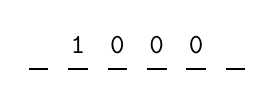
\begin{tikzpicture}
        \foreach \x[count=\i] in {, 1, 0, 0, 0, } {
            \draw[thick] (\i*0.5-0.25, 0) -- (\i*0.5, 0);
            \node at (\i*0.5-0.125, 0.3) {\texttt{\x}};
        }
    \end{tikzpicture}
    \caption{A TM tape on $\{0, 1\}$.}
    \label{fig:tml_tape_example}
\end{figure}
 
We will now illustrate this process. We execute the program \texttt{isEven} on the tape at Figure \ref{fig:tml_tape_example}.
\begin{itemize}
    \item Initially, the tape is the given tape; the current block is at lines 5-15; and the tapehead index is $0$, with value $1$.
    
    \item Since the tapehead value is \texttt{1}, the basic block to be executed is lines 5-7. Hence,
    \begin{itemize}
        \item the tape remains unchanged;
        \item the current block is still at lines 5-15; and
        \item and the tapehead index becomes $1$, with value \texttt{0}.
    \end{itemize}
    
    \item The transition for \texttt{0} and \texttt{1} are the same with respect to the current block. This means that we keep moving to the right until we end up at a blank symbol. At that point, the following is the state of the tape:
    \begin{figure}[H]
        \centering
        \begin{tikzpicture}
            \foreach \x[count=\i] in {, 1, 0, 0, 0, } {
                \draw[thick] (\i*0.5-0.25, 0) -- (\i*0.5, 0);
                \node at (\i*0.5-0.125, 0.3) {\texttt{\x}};
            }
            \draw[->] (2.875, -0.5) -- (2.875, -0.1);
        \end{tikzpicture}
    \end{figure}
    The arrow points at the tapehead value. We are still executing the same block, and the tape has not been altered.
    
    \item Now, since the tapehead value is \texttt{blank}, we move to the left. Moreover, the current block is at lines 10-14. The tape has still not been changed. The current value is now $0$.

    \item The tapehead value is currently \texttt{0}. So,  
    \begin{itemize}
        \item the tape value changes to \texttt{blank};
        \item we have reached the \texttt{accept} command; and
        \item the tapehead pointer move to the left (by default), to index $2$.
    \end{itemize}
    Hence, execution terminates, with result accept and the following tape state:
    \begin{figure}[H]
        \centering
        \begin{tikzpicture}
            \foreach \x[count=\i] in {, 1, 0, 0, , } {
                \draw[thick] (\i*0.5-0.25, 0) -- (\i*0.5, 0);
                \node at (\i*0.5-0.125, 0.3) {\texttt{\x}};
            }
            \draw[->] (1.875, -0.5) -- (1.875, -0.1);
        \end{tikzpicture}
    \end{figure}
\end{itemize}

\chapter{Proof of Equivalence}
In this chapter, we give a proof of equivalence between TMs and TML programs. This is done in many steps that involve:
\begin{itemize}
    \item proving that a TM can be converted to a complete TML program;
    \item proving that a complete TML program can be converted to a TM; and
    \item proving that a valid TML program can be converted to a complete TML program.
\end{itemize}

\section{Complete TML Programs}
When we defined execution of a valid TML program on a tape in the specification, we said that a basic block need not have all 3 types of commands (\textit{changeto}, \textit{move} and a \textit{flow} command), but in the execution above, we have established some `default' ways in which a program gets executed. In particular,
\begin{itemize}
    \item if the \textit{changeto} command is missing, we do not change the value of the tape;
    \item if the \textit{move} command is missing, we move left;
    \item if the \textit{flow} command is missing, we can establish what to do using the rules described above- this is a bit more complicated than the two commands above.
\end{itemize}
Nonetheless, it is possible to include these `default' commands to give a \emph{complete} version of the program. This is what we will establish in this section. 

Consider the following complete program.
\lstinputlisting[language=TML]{code/complete_tml.txt}
Now, we consider the rules that a complete TML program obeys:
\begin{itemize}
    \item A basic block in a complete program has all the necessary commands- if the basic block is inside \textit{while} case, it has a \textit{changeto} command and a \textit{move} command; otherwise, it also has a \textit{flow} command.
    \item A module in a complete program is composed of a single switch block.
\end{itemize}

% By adding the `default' values for the \textit{changeto} and the \textit{move} command, we can partly complete a valid TML program. We can further break 
We will now construct a complete TML program for a valid TML program.
\begin{enumerate}
    \item We first break each module into smaller modules so that every module has just one basic/switch block- we add a \textit{goto} command to the next module if it appeared just below this block.
    \item Then, we can convert each basic block to a switch block by just adding a single case that applies to each letter in the alphabet.
    \item Finally, we add the default values to each basic block to get a complete TML program.
\end{enumerate}
This way, we can associate every block in the valid program with a corresponding block in the complete program. The complete version is always a switch block and might have more commands than the original block, but it still has all the commands present in the original block. 

We now illustrate this process with an example. Assume we first have the following program.
\lstinputlisting[language=TML]{code/complete_program_0.txt}
In step 1 of the completion process, we create a module for each block. In this program, there are two basic blocks- at lines 3-4 and 5-6. So, after applying the first step, we get the following program.
\lstinputlisting[language=TML]{code/complete_program_1.txt}
In this case, we have two basic blocks at lines 3-5 and 8-9. So, in step 2, we convert them into switch blocks and get the following program.
\lstinputlisting[language=TML]{code/complete_program_2.txt}
Finally, we add all the default values in step 3 and get the following program.
\lstinputlisting[language=TML]{code/complete_program_3.txt}
This program obeys the definition of a complete program.

\begin{theorem} \label{thm:complete_TM}
    Let $P$ be a valid TML program. Then, $P$ and its completion $P^+$ execute on every tape $T$ in the same way. That is,
    \begin{itemize}
        \item for every valid index $n$, if we have tape $T_n$, tapehead index $i_n$ and module $m_n$ with executing block $b_n$ for the TML program $P$, and we have tape $S_n$, tapehead index $j_n$ and module $t_n$, then $T_n = S_n$, $i_n = j_n$, and $t_n$ is the corresponding complete module block of $b_n$;
        \item $P$ terminates execution on $T$ if and only if $P^+$ terminates execution on $T$, with the same final status (\texttt{accept} or \texttt{reject}).
    \end{itemize}
\end{theorem}
\begin{proof}
    We prove this by induction on the execution step (of the tape). 
    \begin{itemize}
        \item At the start, we have the same tape $T$ for both $P$ and $P^+$, with tapehead index 0. Moreover, the corresponding (completed) module of the first block in the first module of $P$ is the first module of $P$. So, the result is true if $n = 0$. 
        \item Now, assume that the result is true for some integer $n$, where the block $b_n$ in the TML program $P$ does not end with a terminating \textit{flow} command. Let $\sigma_n$ be the letter at index $i_n = j_n$ on the tape $S_n = T_n$.
        \begin{itemize}
            \item If the \textit{changeto} command is missing in $b_n$ for $\sigma_n$, then the next tape $T_{n+1} = T_n$. In the complete module $m_n$, the case for $\sigma_n$ will have the command \texttt{changeto} $\sigma_n$. So, the next tape is given by:
            \[S_{n+1}(x) = \begin{cases}
                S_n(x) & x \neq j_n \\
                \sigma_n & \text{otherwise}
            \end{cases}.\]
            Therefore, we have $S_{n+1} = S_n$ as well. So, $T_{n+1} = S_{n+1}$. Otherwise, we have the same \textit{changeto} command in the two blocks, in which case $T_{n+1} = S_{n+1}$ as well.
            
            \item If the \textit{move} command is missing in $b_n$ for $\sigma_n$, then the next tapehead index $i_{n+1} = i_n - 1$. In the complete module $m_n$, the case for $\sigma_n$ will have the command \texttt{move left}, so we also have $j_{n+1} = j_n - 1$. Applying the inductive hypothesis, we have $i_{n+1} = j_{n+1}$. Otherwise, we have the same \textit{move} command, meaning that $i_{n+1} = j_{n+1}$ as well.
            
            \item We now consider the next block $b_{n+1}$:
            \begin{itemize}
                \item If the block $b_n$ is a \textit{switch} block with a \textit{while} case for $\sigma_n$, then this is still true in the module $m_n$. So, the next block to be executed in $P$ is $b_n$, and the next module to be executed in $P^+$ is $m_n$. In that case, the corresponding module of the block $b_{n+1} = b_n$ is still $m_{n+1} = m_n$.
    
                \item Instead, if the block $b_n$ has no \textit{flow} command for $\sigma_n$, and is not the last block, then the next block to execute is the block just below $b_n$, referred as $b_{n+1}$. By the definition of $P^+$, we find that the case block in the module $m_n$ has a \textit{goto} command, going to the module $m_{n+1}$ which corresponds to the block $b_{n+1}$. 
            
                \item Now, if the \textit{flow} command is missing for $\sigma_n$ and this is the last block, then execution is terminated with the status \texttt{reject} for the program $P$. In that case, the case for $\sigma_n$ in the module $m_n$ has the \texttt{reject} command present, so the same happens for $P^+$ as well. 
            
                \item Otherwise, both $P$ and $P^+$ have the same flow command, meaning that there is either correspondence between the next module to be executed, or both the program terminate with the same status. 
            \end{itemize}
        \end{itemize}
    \end{itemize}
    In that case, $P$ and $P^+$ execute on $T$ the same way by induction.
\end{proof}

\section{Equivalence of TMs and TMLs}
In this section, we will show that there is an equivalence between TMs and valid TML programs. We will first construct a valid TML program for a TM and then show that it has the same behaviour as the TM. Later, we will construct a TM for a TML program, and show the equivalence in this case as well.

\begin{figure}[htb]
    \centering
    \begin{tikzpicture}
        \node[state, accepting] (q1) at (2.5, 0) {$q_0$};
        \node[state, fill=green, opacity=0.6] (A) at (5, -1) {$A$};
        \node[state, fill=red, opacity=0.6] (R) at (5, 1) {$R$};

        \draw[->] (q1) edge[loop above] node[above] {$1, R$} (q1);
        \draw[->] (q1) -- node[below, rotate=-20] {$0, R$} (A);
        \draw[->] (q1) -- node[above, rotate=20] {$\#, R$} (R);
    \end{tikzpicture}
    \caption{A TM that accepts binary strings containing 0}
    \label{fig:simple_tm}
\end{figure}
We will first illustrate how to convert a TM to a (complete) TML program. So, consider the TM at Figure \ref{fig:simple_tm}. Then, its corresponding TML program is the following:
\lstinputlisting[language=TML]{code/tm_to_tml.txt}
In general, we convert each (non-terminating) state in the TM $M$ to a TML module. The following is how we create the module:
\begin{itemize}
    \item the module contains a single \textit{switch} command;
    \item for each letter $\sigma$ in the alphabet $\Sigma^+$, denote $\delta(q, \sigma) = (q', \sigma', \texttt{dir})$. We add an \textit{if} case in the \textit{switch} command corresponding to letter $\sigma$ with the following commands:
    \begin{itemize}
        \item \texttt{changeto} $\sigma'$
        \item \texttt{move} \textit{dir}
        \item if $q'$ is \texttt{accept}, then the command \texttt{accept}; if $q'$ is \texttt{reject}, then the command \texttt{reject}; otherwise, \texttt{goto} $q'$.
    \end{itemize}
\end{itemize}
Moreover, we can construct the program $P$ with:
\begin{itemize}
    \item the alphabet $\Sigma$;
    \item modules corresponding to every state $q$ in $M$;
    \item the module corresponding to the initial state $q_0$ placed at the top.
\end{itemize}
We say that $P$ is the \emph{corresponding program for $M$}.

\begin{theorem} \label{thm:TM_to_TMP}
    Let $M$ be a TM, and let $P$ be the corresponding program for $M$. Then, $M$ and $P$ execute on every tape $T$ in the same way. That is, 
    \begin{itemize}
        \item for every valid index $n$, if we have tape $T_n$, tapehead index $i_n$ and module $m_n$ for the TML program $P$, and we have tape $S_n$, tapehead index $j_n$ and state $q_n$ for the TM $M$, then $T_n = S_n$, $i_n = j_n$ and $m_n$ is the corresponding module for $q_n$;
        \item $M$ terminates execution on $T$ if and only if $P$ terminates execution on $T$, with the same final status (\texttt{accept} or \texttt{reject}).
    \end{itemize}
\end{theorem}
\begin{proof}
    We prove this by induction on the execution step. 
    \begin{itemize}
        \item At the start, we have the same tape $T$ for both $M$ and $P$, with tapehead index $0$. Moreover, the first module in $P$ corresponds to the initial state $q_0$. So, the result is true if $n = 0$.
        
        \item Now, assume that the result is true for some integer $n$, where the TM state $q_n$ is not \texttt{accept} or \texttt{reject}. In that case, $T_n = S_n$, $i_n = j_n$ and $m_n$ is the corresponding module for $q_n$. Let $\sigma_n$ be the letter at index $i_n = j_n$ on the tape $T_n = S_n$. Denote $q(q_n, \sigma_n) = (q_{n+1}, \sigma_{n+1}, \texttt{dir})$. In that case,
        \[T_{n+1}(x) = \begin{cases}
            T_n(x) & x \neq i_n \\
            \sigma_{n+1} & \text{otherwise},
        \end{cases} \qquad i_{n+1} = \begin{cases}
            i_n - 1 & \texttt{dir} = \texttt{left} \\
            i_n + 1 & \texttt{dir} = \texttt{right},
        \end{cases}\]
        and the next state is $q_{n+1}$. 
        
        \begin{itemize}
            \item We know that the module $m_n$ in TML program $P$ corresponds to the state $q_n$, so it has a \texttt{changeto} $\sigma_{n+1}$ command for the case $\sigma_n$. In the case, the next tape for $P$ is:
            \[S_{n+1}(x) = \begin{cases}
                S_n(x) & x \neq i_n \\
                \sigma_{n+1} & \text{otherwise}.
            \end{cases}\]
            So, $T_{n+1} = S_{n+1}$. 
            
            \item Similarly, the case also contains a \texttt{move dir} command. This implies that the next tapehead index for $P$ is:
            \[j_{n+1} = \begin{cases}
                j_n - 1 & \texttt{dir} = \texttt{left} \\
                j_n + 1 & \texttt{dir} = \texttt{right}.
            \end{cases}\]
            Hence, $i_{n+1} = j_{n+1}$. 
        
            \item Next, we consider the value of $q_{n+1}$:
            \begin{itemize}
                \item If $q_{n+1} = q_n$, then the case block is a \textit{while} block, and vice versa. So, the next module to be executed is $m_n$. In that case, $m_{n+1}$ still corresponds to $q_{n+1}$.
                \item Otherwise, we have an \textit{if} block. 
                \begin{itemize}
                    \item In particular, if $q_{n+1}$ is the \texttt{accept} state, then the case for $\sigma_n$ contains the \textit{flow} command \texttt{accept}, and vice versa. In that case, execution terminates with the same final status of \texttt{accept}. The same is true for \texttt{reject}. 
                    \item Otherwise, the module contains the command \texttt{goto} $m_{n+1}$, where $m_{n+1}$ is the corresponding module for $q_{n+1}$.
                \end{itemize}
            \end{itemize}
        \end{itemize}
        % Therefore, if the result holds for $n$, it holds for $n+1$. So, the result follows from induction.
    \end{itemize}
    In that case, $P$ and $M$ execute on $T$ the same way by induction.
\end{proof}

Next, we construct a TM for a TML program. This process is essentially the inverse of the one we saw converting a TML program to a TM. In particular, for each module $m$ in $P$, we construct the state $q$ as follows- for each letter $\sigma$ in $\Sigma^+$, we define $\delta(q, \sigma) = (q', \sigma', \texttt{dir})$, where:
\begin{itemize}
    \item the value $\sigma'$ is the letter given in the \textit{changeto} command within $m$;
    \item the value \texttt{dir} is the direction given in the \textit{move} command within $m$;
    \item if the \textit{flow} command in $m$ corresponding to $\sigma$ is \texttt{accept}, then $q'$ is the \texttt{accept} state; if it is \texttt{reject}, then $q'$ is the \texttt{reject} state; if we are in a \textit{while} block, then $q' = q$; otherwise, $q'$ is the state corresponding to the module given in the \textit{goto} command.
\end{itemize}
Then, the TM with all the states $q$, the same alphabet $\Sigma$, the transition function $\delta$ and initial state $q_0$ corresponding to the first module in $P$ is the \emph{corresponding TM for $P$}. 

\begin{figure}[htb]
    \centering
    \begin{tikzpicture}
        \node[state, accepting] (s0) at (-0.5, 0) {$q_0$};
        \node[state] (s1) at (2, 0) {$q_1$};
        \node[state] (s2) at (4, 1) {$q_2$};
        \node[state, fill=green, opacity=0.6] (A) at (6, 1) {$A$};
        \node[state, fill=red, opacity=0.6] (R) at (6, -1) {$R$};
        
        \draw[-stealth] (s0) edge[loop above] node {$a|b, R$} (s0);
        \draw[-stealth] (s0) -- node[above] {$\#, L$} (s1);

        \draw[-stealth] (s1) -- node[above, rotate=25] {$a, L$} (s2);
        \draw[-stealth] (s1) -- node[below, rotate=-15, pos=0.4] {$\#, L$} (R);
        \draw[-stealth] (s1) -- node[above, rotate=-15, pos=0.4] {$b \to \#, L$} (R);

        \draw[-stealth] (s2) -- node[above] {$\#, L$} (A);

        \draw[-stealth] (s2) -- node[above, rotate=-45] {$b \to \#, L$} (R);
        \draw[-stealth] (s2) -- node[below, rotate=-45] {$\#, L$} (R);
    \end{tikzpicture}
    \caption{The TM corresponding to the program above. The state $q_0$ corresponds to the module \texttt{moveToEnd}; the state $q_1$ corresponds to the module \texttt{checkAFirst}; and the state $q_2$ corresponds to the module \texttt{checkASecond}.}
    \label{fig:tm_from_tml}
\end{figure}

We now illustrate this process with an example. So, consider the following TML program:
\lstinputlisting[language=TML]{code/tml_to_tm.txt}
Then, its corresponding TM is given in Figure \ref{fig:tm_from_tml}.
\begin{theorem}
    Let $P$ be a TML program, and let $M$ be the corresponding TM for $P$. Then, $P$ and $M$ execute on every tape $T$ in the same way. That is,
    \begin{itemize}
        \item for every valid index $n$, if we have tape $T_n$, tapehead index $i_n$ and module $m_n$ for TML program $P$, and we have tape $S_n$, tapehead index $j_n$ and state $q_n$ for the TM $M$, then $T_n = S_n$, $i_n = j_n$ and $q_n$ is the corresponding state for $m_n$;
        \item $P$ terminates execution on $T$ if and only if $M$ terminates execution on $T$, with the same final status (\texttt{accept} or \texttt{reject}).
    \end{itemize}
\end{theorem}
\begin{proof}
    Without loss of generality, assume that $P$ is complete. We prove this as well by induction on the execution step of the tape. 
    \begin{itemize}
        \item At the start, we have the same tape $T$ for both $P$ and $M$, with tapehead index $0$. Moreover, the initial state $q_0$ in $M$ corresponds to the first module in $P$. So, the result is true if $n = 0$. 
        
        \item Now, assume that the result is true for some integer $n$, which is not the terminating step in execution. In that case, $S_n = T_n$, $j_n = i_n$ and $q_n$ is the corresponding state for $m_n$. Let $\sigma_n$ be the letter at index $j_n = i_n$ on the tape $S_n = T_n$. We now consider the single switch block in $m_n$:
        \begin{itemize}
            \item If the block in $m_n$ corresponding to $\sigma_n$ is a \textit{while} block, then we know that its body is partially complete, and so is composed of the following commands:
            \begin{itemize}
                \item \texttt{changeto} $\sigma_{n+1}$
                \item \texttt{move dir}
            \end{itemize}
            So, we have $\delta(q_n, \sigma_n) = (q_n, \sigma_{n+1}, \texttt{dir})$. Using the same argument as in Theorem \ref{thm:TM_to_TMP}, we find that $T_{n+1} = S_{n+1}$ and $i_{n+1} = j_{n+1}$. Also, $q_{n+1} = q_n$ is the corresponding state for $m_{n+1} = m_n$. 
            
            \item Otherwise, we have an \textit{if} command. In this case, the case body is complete, and so composed of the following commands:
            \begin{itemize}
                \item \texttt{changeto} $\sigma_{n+1}$
                \item \texttt{move dir}
                \item \texttt{accept}, \texttt{reject} or \texttt{goto} $m_{n+1}$.
            \end{itemize}
            So, we have $\delta(q_n, \sigma_n) = (q_{n+1}, \sigma_{n+1}, \texttt{dir})$, where $q_{n+1}$ is the corresponding state to the \textit{flow} command present. Here too, we have $T_{n+1} = S_{n+1}$ and $i_{n+1} = j_{n+1}$ by construction. 
        \end{itemize}
        Now, we consider the flow command:
        \begin{itemize}
            \item If we have an \texttt{accept} command in the body, then $q_{n+1}$ is the accepting state, and vice versa. So, we terminate execution with the final status of \texttt{accept}. The same is true for \texttt{reject}. 
            \item Otherwise, the state $q_{n+1}$ is the corresponding state to the module $m_{n+1}$.
        \end{itemize}
        In all cases, there is a correspondence between the state for $m_{n+1}$ and $q_{n+1}$.   
    \end{itemize}
    So, the result follows from induction.
\end{proof}

Hence, we have established that for any valid TML program, there is a TM, and vice versa.

\section{TML as a model of computation}
Since TML programs and TMs are equivalent, this implies that TML programs are a model for computation. Note that while we have given a proof for equivalence for TMs, this representation is based on accepting and rejecting programs only. Not all TMs are of this form. In particular, it is also possible for a TM to halt instead of accepting or rejecting.

Although the equivalence is limited to a subclass of TMs, we can add another flow command \texttt{halt} that mimics the halting behaviour. However, this is not necessary- we can use the accept state (or equally the reject state) to mimic the behaviour of halting. Since accepting or rejecting results in the program halting, we can simply disregard the final result, and possibly read the output from the tape to infer the actual result.

\chapter{Product Screenshots}
In this chapter, we illustrate some screenshots of the website.

\section{Homepage}
\begin{figure}[htb]
    \centering
    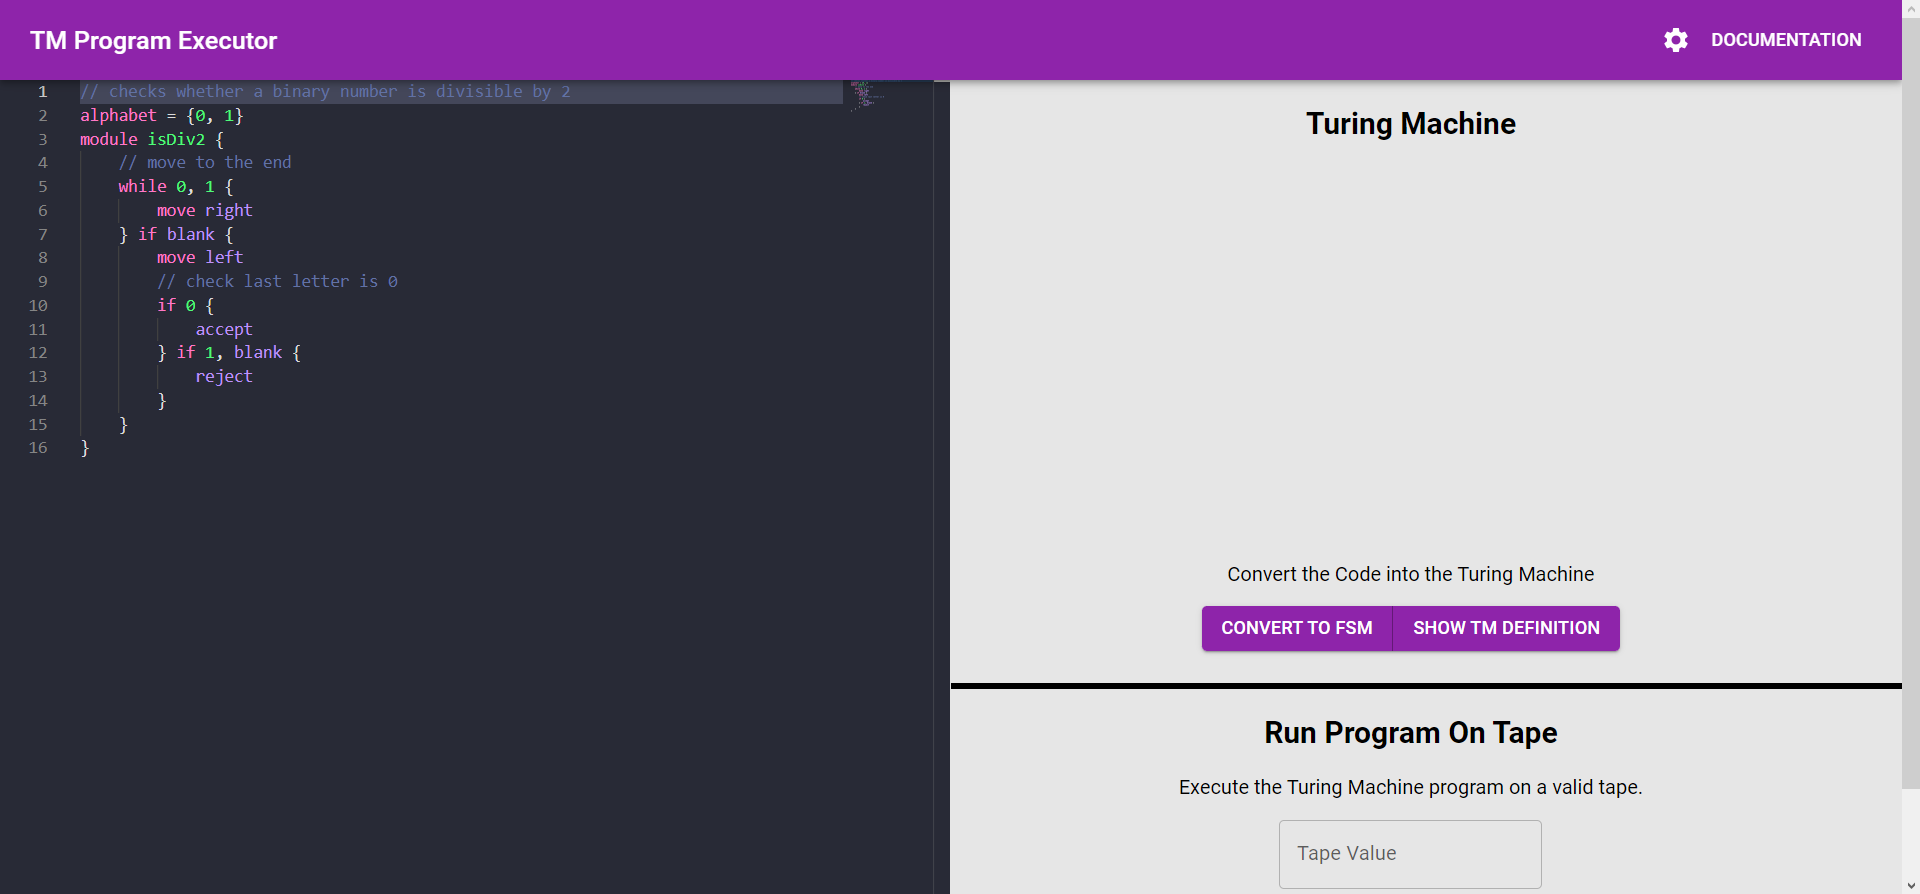
\includegraphics[scale=0.18]{images/Homepage at start.png}
    \caption{The initial rendering of the homepage.}
    \label{fig:homepage_initial}
\end{figure}
The initial rendering of the homepage is given in Figure \ref{fig:homepage_initial}. It shows an example program initially, with no TM conversion or tape execution. We can change the program in settings. The user can press the button in TM panel to convert the program to either the FSM representation or the definition version.

\begin{figure}[htb]
    \centering
    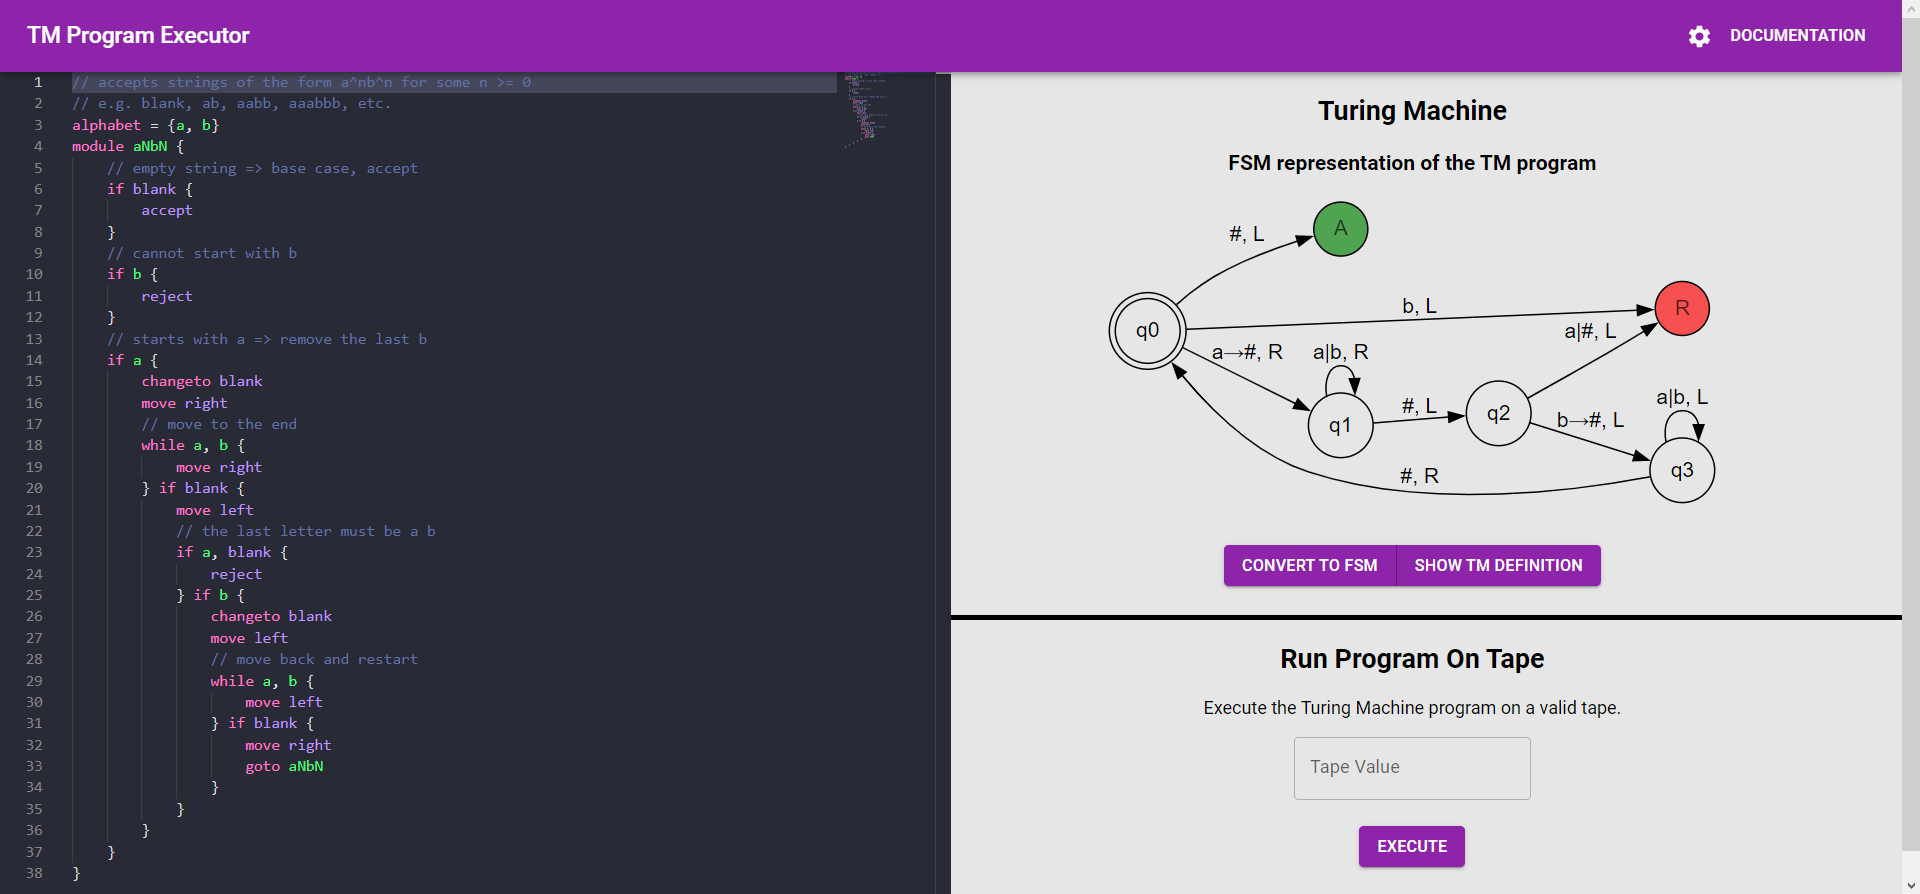
\includegraphics[scale=0.18]{images/Homepage w. TM.png}
    \caption{The homepage after the user converts the TML program into FSM version of TM.}
    \label{fig:homepage_tm_conversion_fsm}
\end{figure}

\begin{figure}[htb]
    \centering
    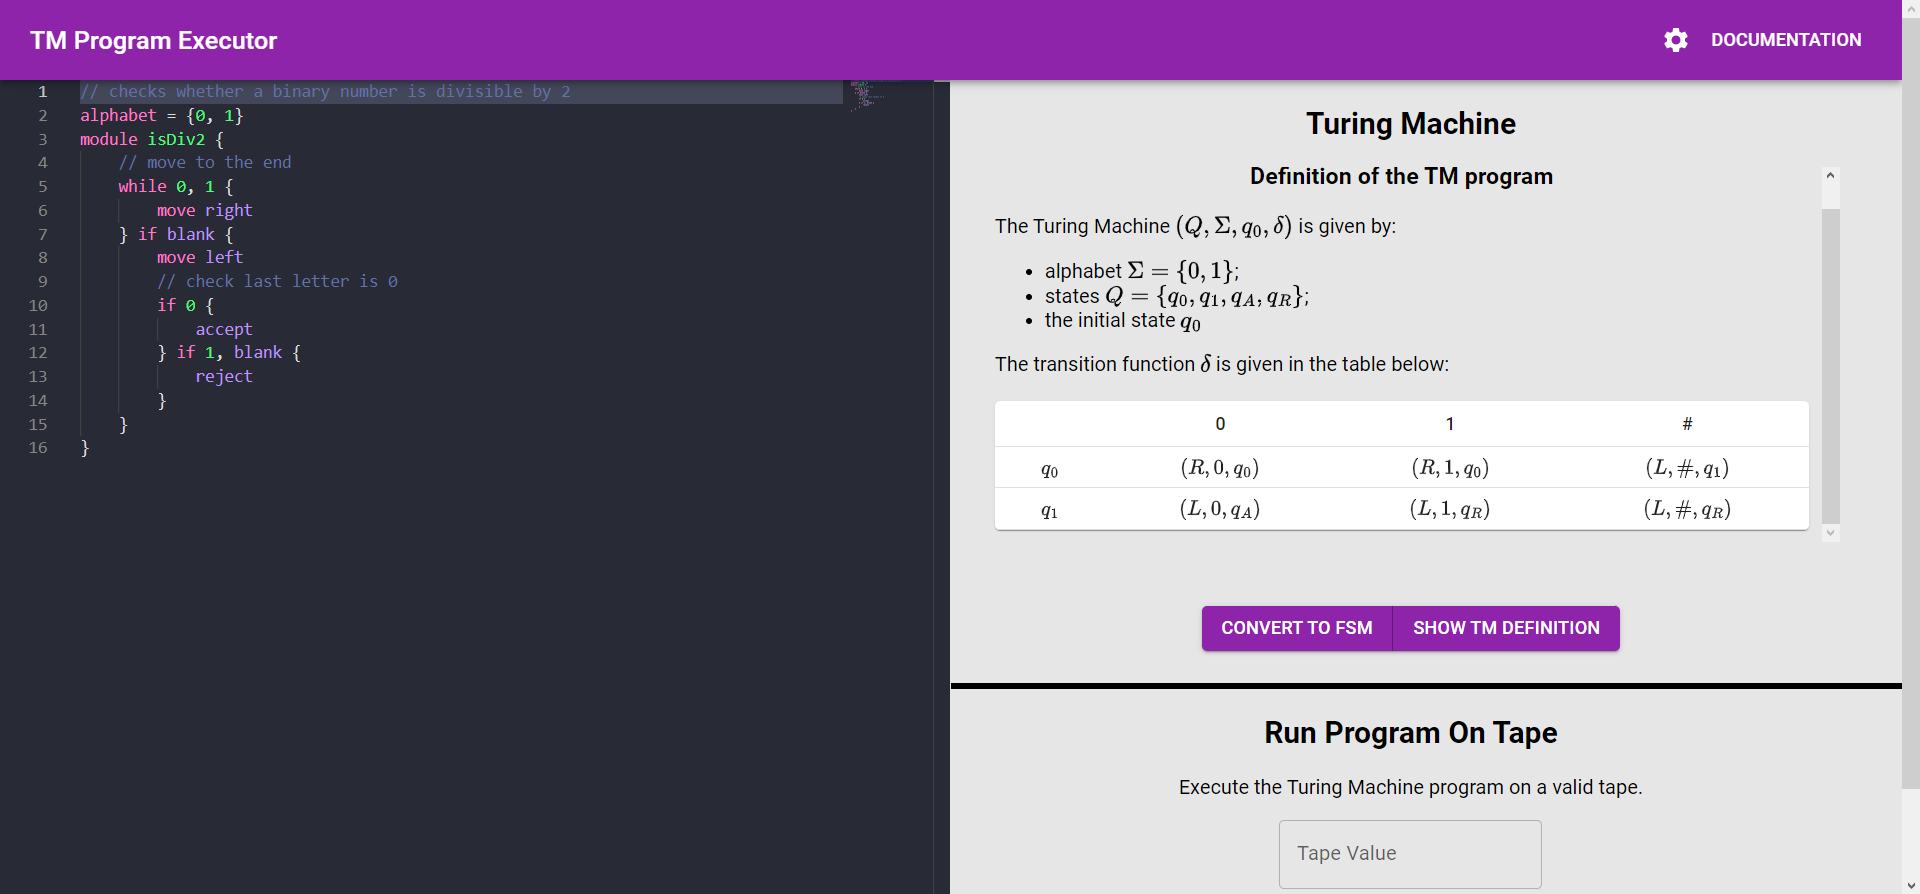
\includegraphics[scale=0.18]{images/Homepage w. TM (def).png}
    \caption{The homepage after the user converts the TML program into definition version of TM}
    \label{fig:homepage_tm_conversion_def}
\end{figure}

Figure \ref{fig:homepage_tm_conversion_fsm} shows the FSM conversion of a TML program on the page, while figure \ref{fig:homepage_tm_conversion_def} shows the definition version.

\begin{figure}[htb]
    \centering
    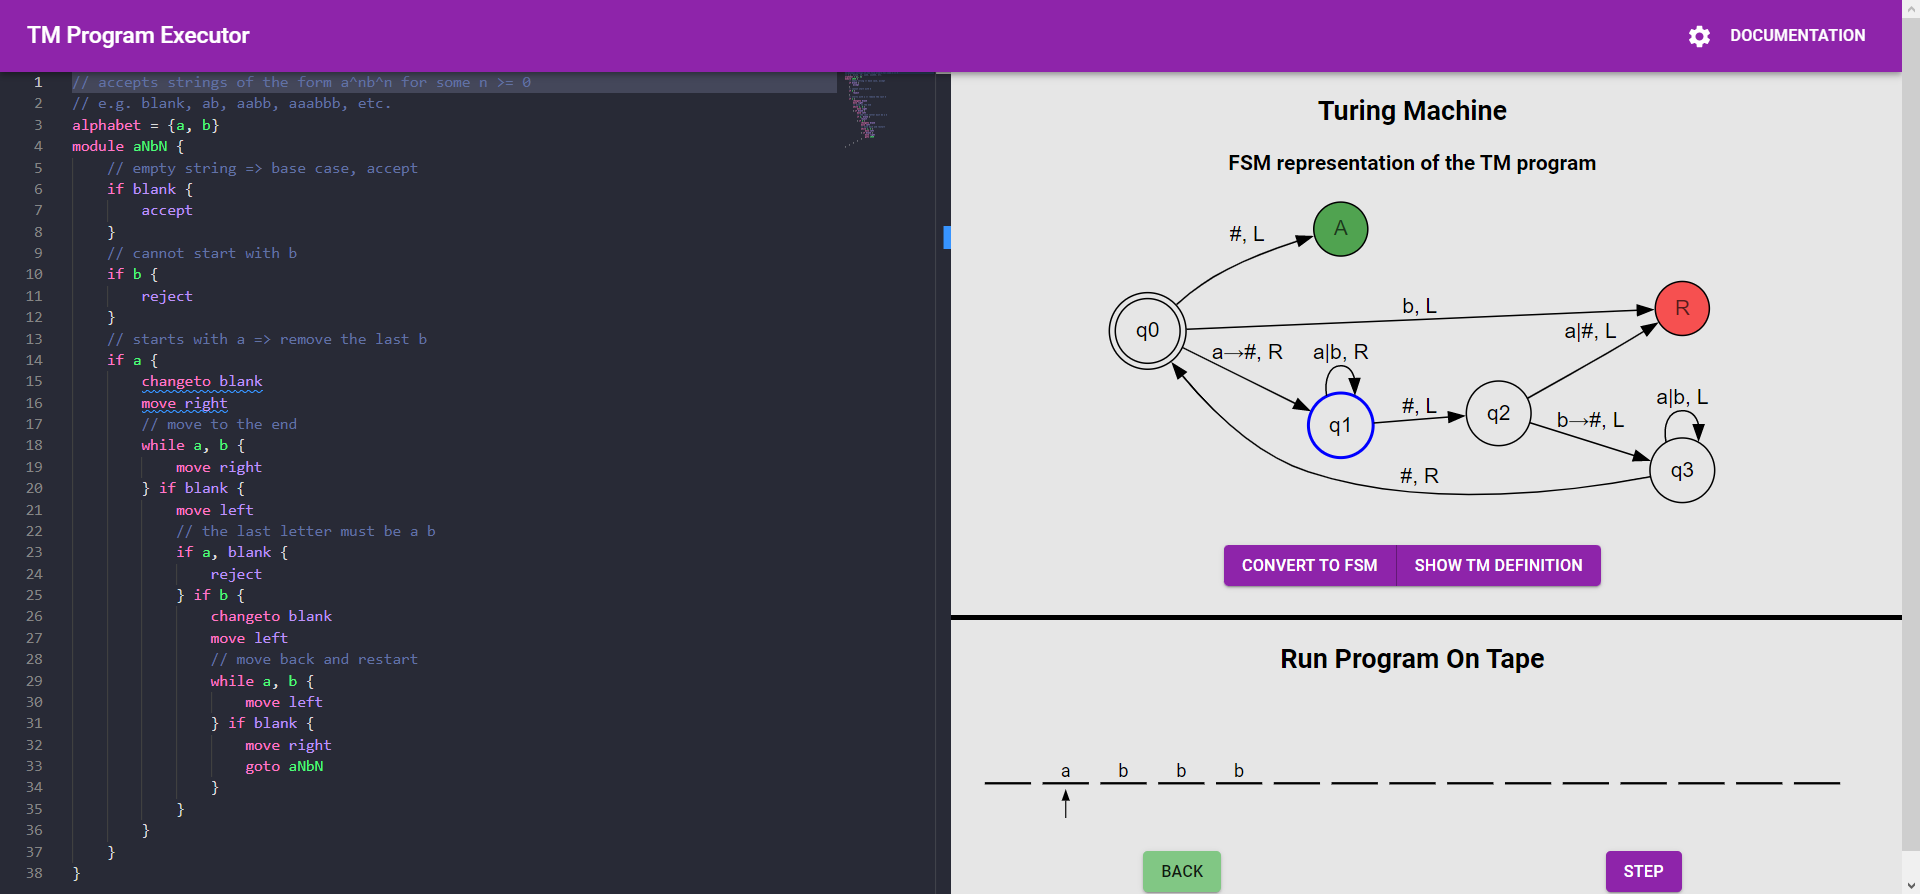
\includegraphics[scale=0.18]{images/Homepage execution start.png}
    \caption{The homepage during tape execution.}
    \label{fig:homepage_execution_start}
\end{figure}

Figure \ref{fig:homepage_execution_start} shows the website during tape execution. The execution is illustrated in code- the current block is highlighted. Moreover, since TM has been converted, the current state is also highlighted in blue.

\newpage

\section{Documentation Pages}
\begin{figure}[htb]
    \centering
    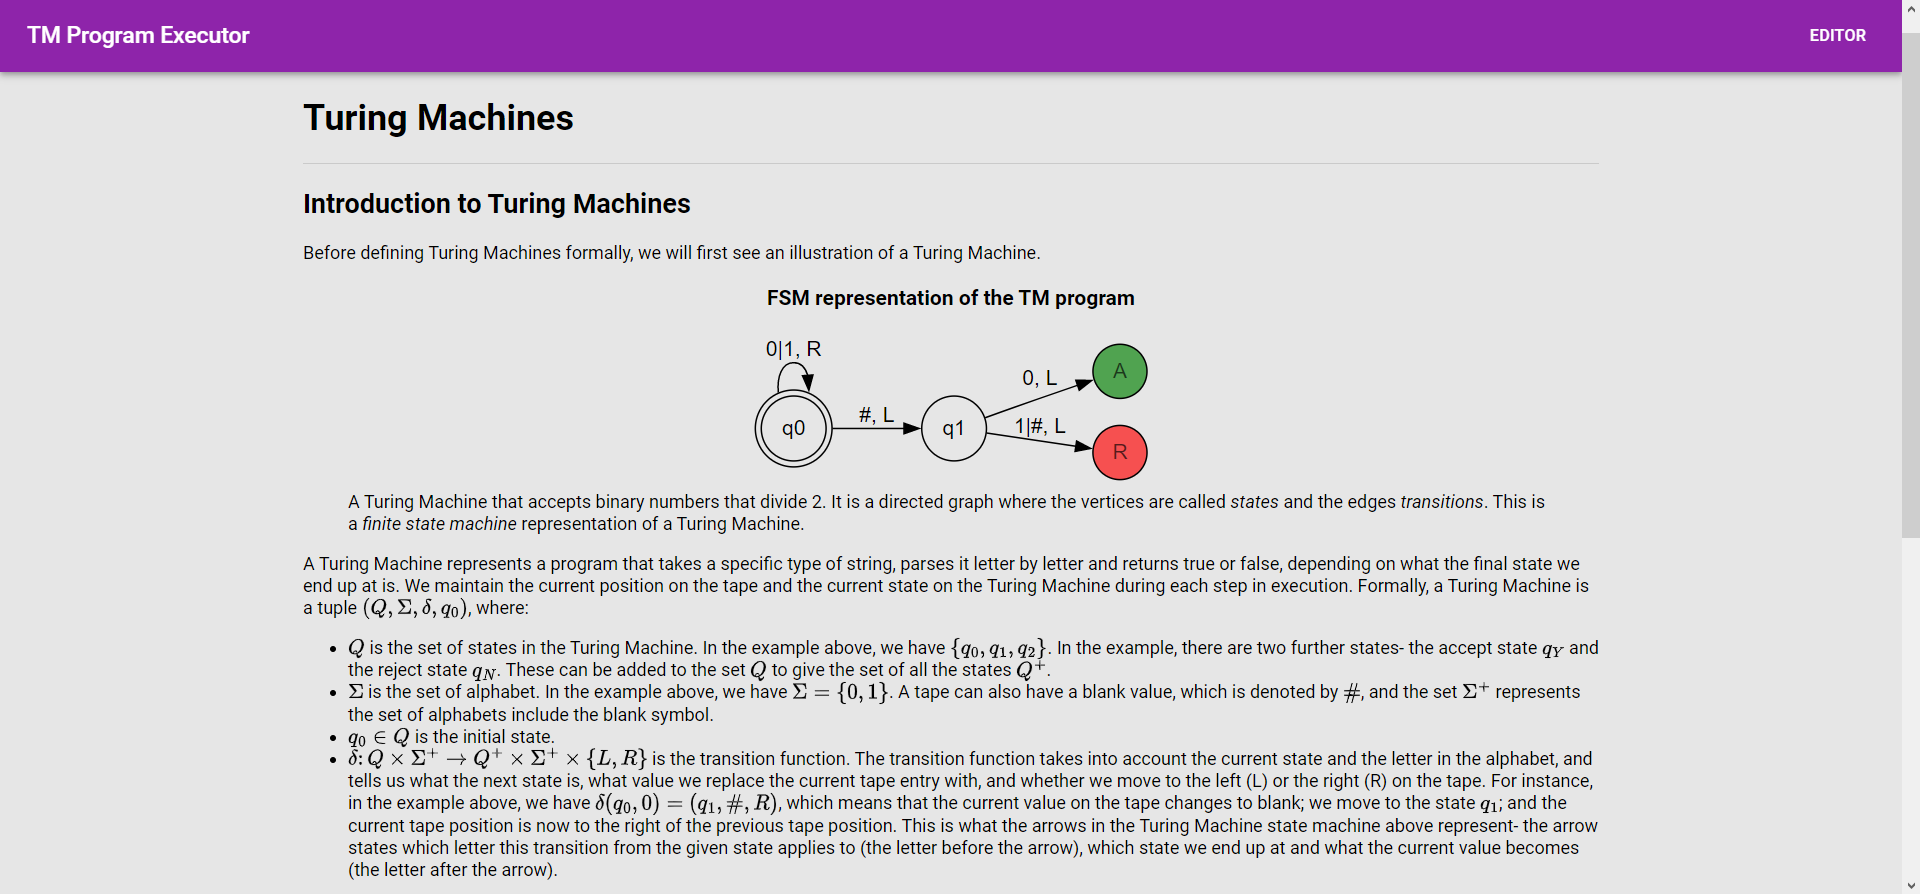
\includegraphics[scale=0.18]{images/Documentation for TM.png}
    \caption{The documentation webpage for TM}
    \label{fig:documentation_tm}
\end{figure}

\begin{figure}[htb]
    \centering
    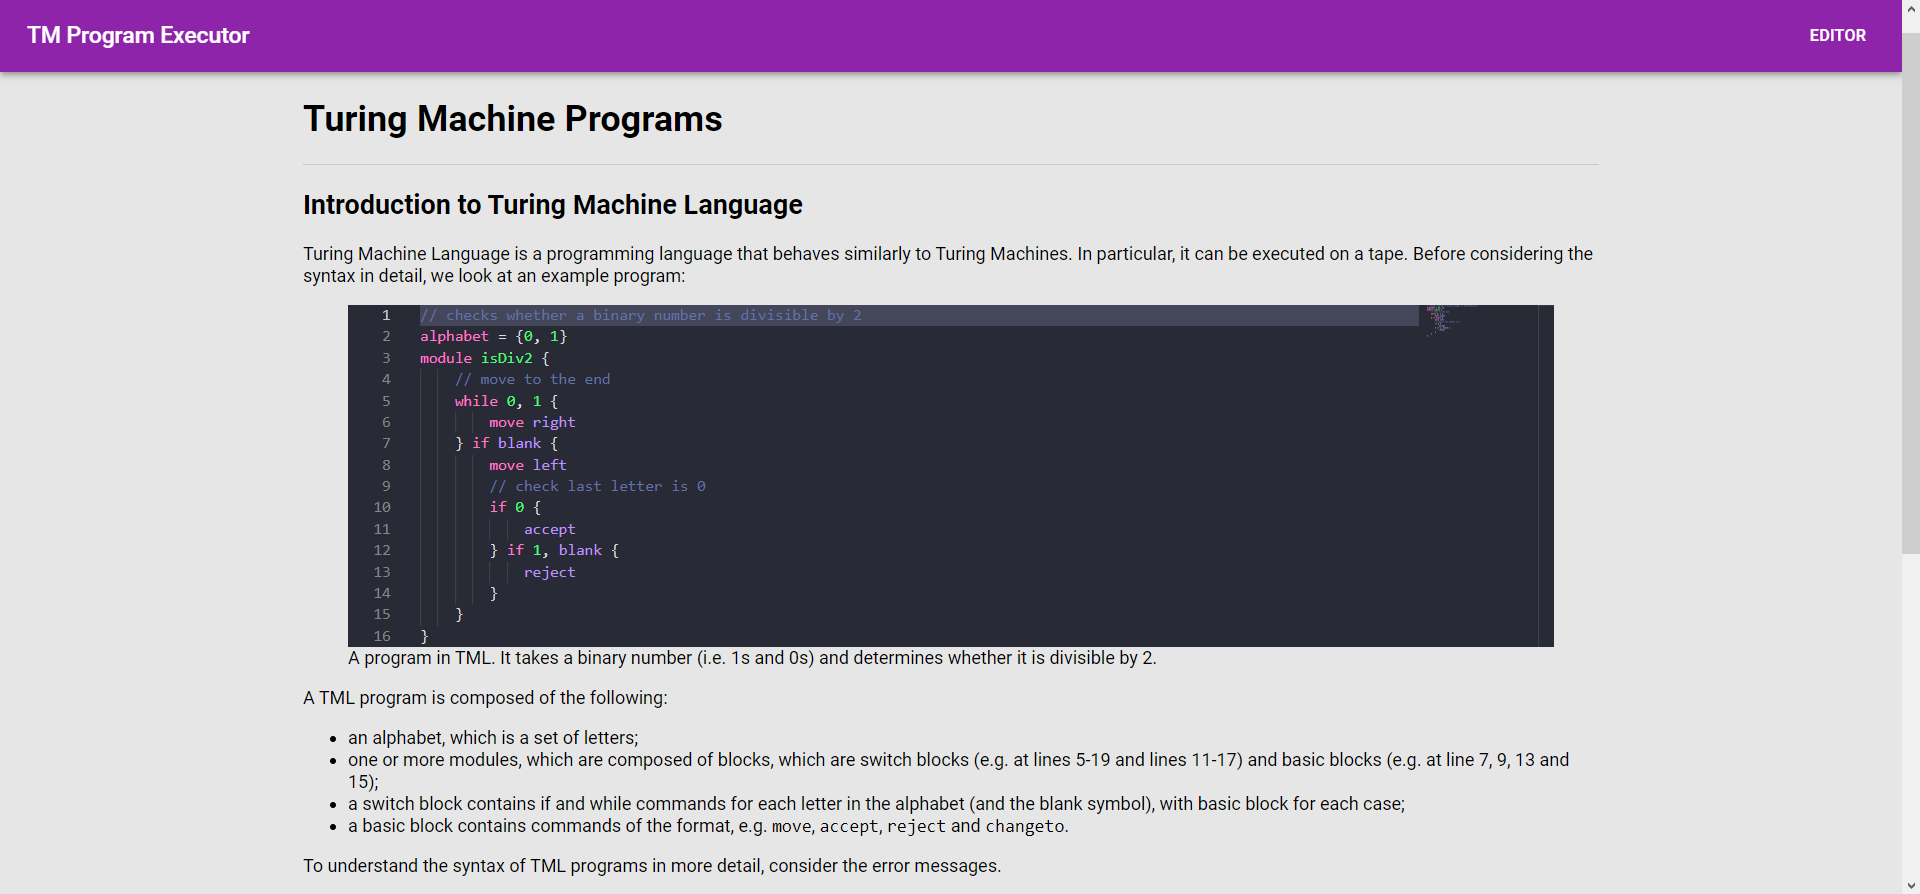
\includegraphics[scale=0.18]{images/Documentation for TML.png}
    \caption{The documentation webpage for TML}
    \label{fig:documentation_tml}
\end{figure}

There are 2 pages in the site dedicated to documentation- one that documents TMs and the other that documents TML. The initial definitions are shown in Figures \ref{fig:documentation_tm} and \ref{fig:documentation_tml}. In each page, there is an example before the actual definition. 

Below the definition, we describe execution on a tape. The user can then execute the TM/TML program by inputting a value. Like in the homepage, different aspects are highlighted during execution to make it easier to follow.

\newpage

\section{Program Error Pages}
There is a specific page in the website that lists all the errors- this is shown in Figure \ref{fig:general_error_page}. The errors are partitioned into 2 groups- parsing/syntax errors and validation errors. 

\begin{figure}[htb]
    \centering
    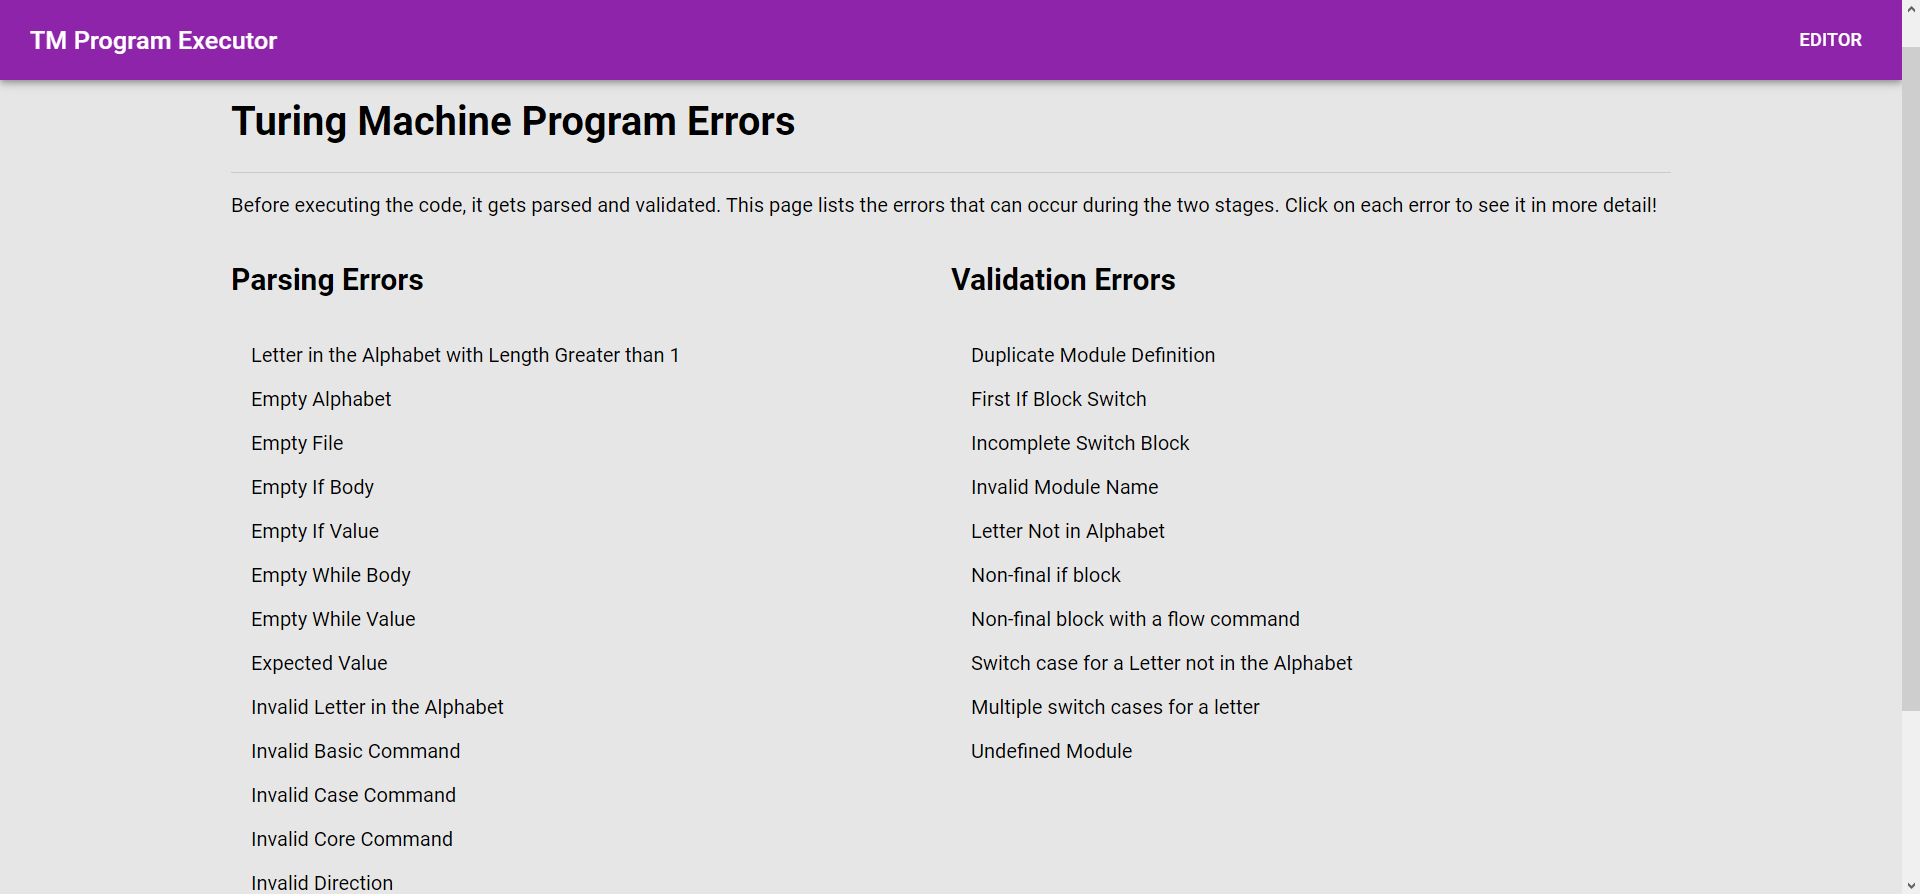
\includegraphics[scale=0.18]{images/General Error Page.png}
    \caption{The general error page that lists all the syntax and validation errors.}
    \label{fig:general_error_page}
\end{figure}

Clicking on an error takes the user to the specific error page. The error page for an undefined module is given in Figure \ref{fig:specific_error_page}. At the top of the webpage is a program that also has this error. We describe the error and then explain how to resolve it.

\begin{figure}[htb]
    \centering
    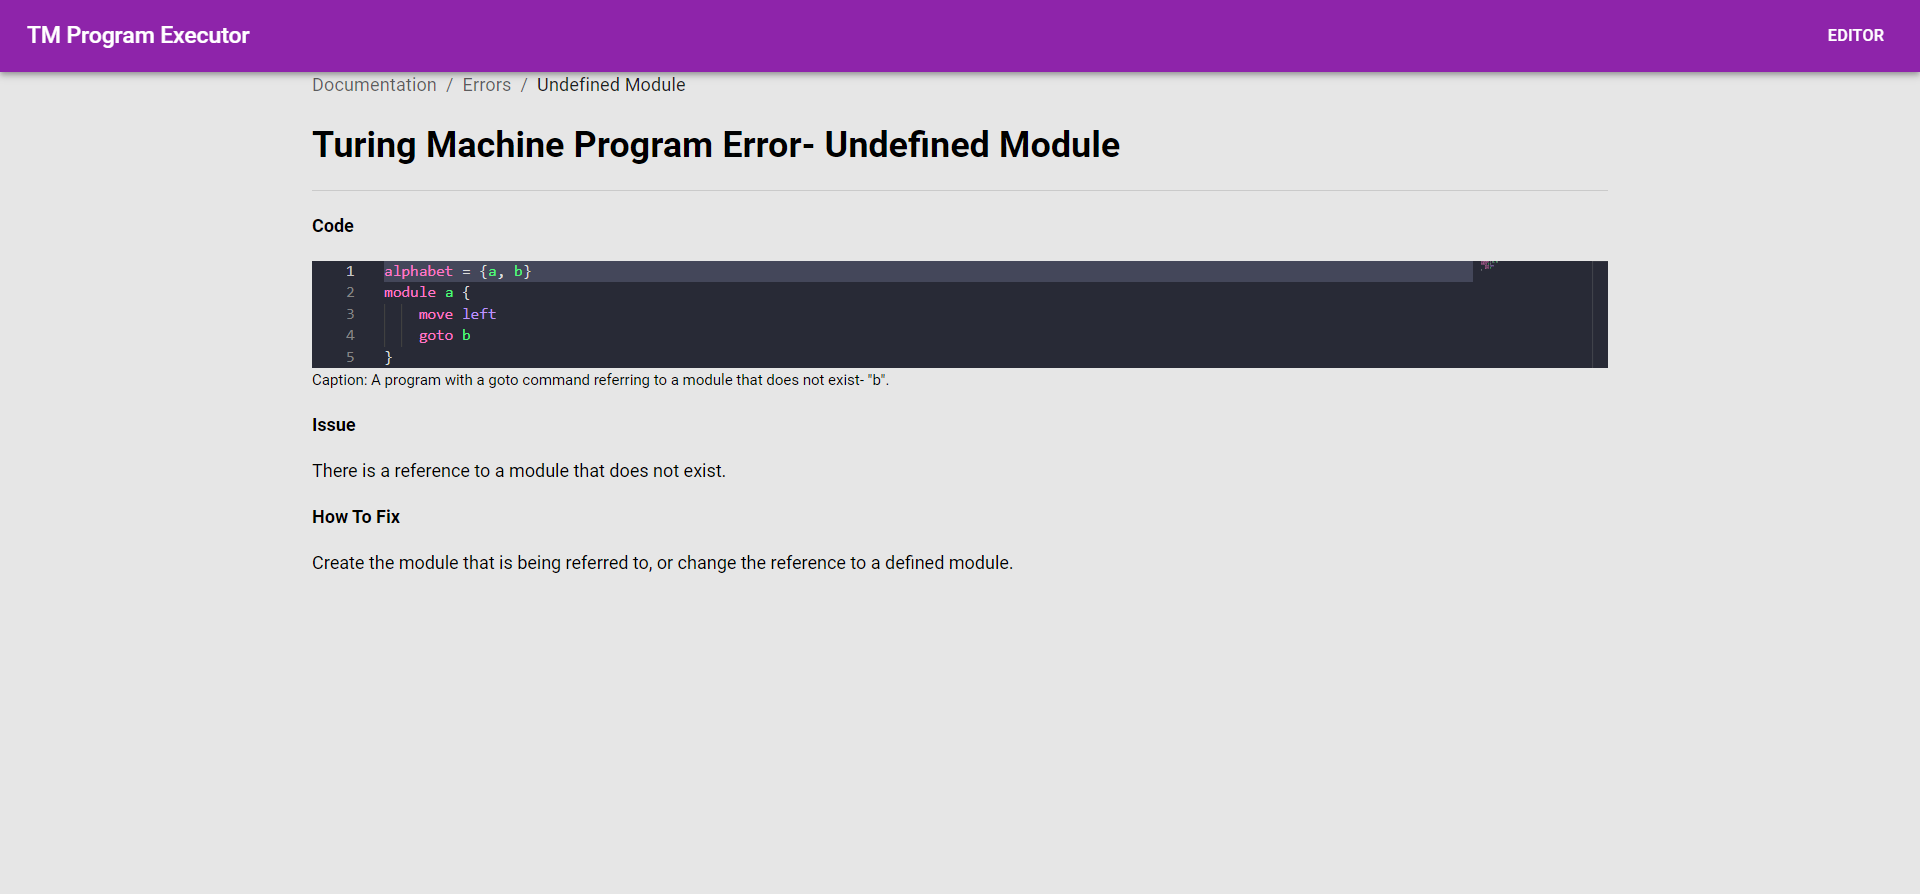
\includegraphics[scale=0.18]{images/Specific Error Page.png}
    \caption{The error page for an undefined module.}
    \label{fig:specific_error_page}
\end{figure}

\chapter{Evaluation Content}
\section{Worksheet}
\subsection{Introduction to Turing Machine Language}
In this section, you are given some programs in Turing Machine Language (TML). They will be used to explain the syntax of the programming language and how they can be run on tapes.
\begin{itemize}
    \item \texttt{isDiv2}:
    \lstinputlisting[language=TML]{code/isDiv2.txt}
    
    \item \texttt{isDiv2Rec}:
    \lstinputlisting[language=TML]{code/isDiv2Rec.txt}

    Both \texttt{isDiv2} and \texttt{isDiv2Rec} correspond to the TM in Figure \ref{fig:corresponding_TM_isDiv2}.
    \begin{figure}[htb]
        \centering
        \begin{tikzpicture}
            \node[state, accepting] (q0) at (0, 0) {$q_0$};
            \node[state] (q1) at (2.5, 0) {$q_1$};
            \node[state, fill=green, opacity=0.6] (A) at (5, -1) {$A$};
            \node[state, fill=red, opacity=0.6] (R) at (5, 1) {$R$};
    
            \draw[->] (q0) edge[loop above] node {$0|1, R$} (q0);
            \draw[->] (q0) -- node[above] {$\#, L$} (q1);
            \draw[->] (q1) -- node[below, rotate=-20] {$0, L$} (A);
            \draw[->] (q1) -- node[above, rotate=20] {$1|\#, L$} (R);
        \end{tikzpicture}
        \caption{The TM for \texttt{isDiv2} and \texttt{isDiv2Rec}.}
        \label{fig:corresponding_TM_isDiv2}
    \end{figure}
    
    \item \texttt{aNbN}:
    \lstinputlisting[language=TML]{code/aNbN.txt}
    The program \texttt{aNbN} corresponds to the TM in Figure \ref{fig:corresponding_TM_aNbN}.
    \begin{figure}[htb]
        \centering
        \begin{tikzpicture}
            \node[state, accepting] (q0) at (0, 0) {$q_0$};
            \node[state] (q1) at (0, -2.5) {$q_1$};
            \node[state] (q2) at (5, -2.5) {$q_2$};
            \node[state] (q3) at (5, 0) {$q_3$};
            \node[state, fill=green, opacity=0.6] (A) at (-2.5, 0) {$A$};
            \node[state, fill=red, opacity=0.6] (R) at (2.5, -1.25) {$R$};

            \draw[->] (q0) -- node[rotate=90, above] {$a \to \#, R$} (q1);
            \draw[->] (q0) -- node[above] {$\#, L$} (A);
            \draw[->] (q0) -- node[below, rotate=-30] {$b, L$} (R);
            \draw[->] (q1) edge[loop left] node {$a|b, R$} (q1);
            \draw[->] (q1) -- node[below] {$\#, L$} (q2);
            \draw[->] (q2) -- node[rotate=90, below] {$b \to \#, L$} (q3);
            \draw[->] (q3) edge[loop right] node {$a|b, L$} (q3);
            \draw[->] (q2) -- node[above, rotate=-30] {$a|\#, L$} (R);
            \draw[->] (q3) -- node[above] {$\#, L$} (q0);
        \end{tikzpicture}
        \caption{The TM for \texttt{aNbN}.}
        \label{fig:corresponding_TM_aNbN}
    \end{figure}
    
\end{itemize}

\subsection{Identifying TML Programs}
In this section, you are presented with TML programs. You will be given some tape values to run the program in and decode what values the program accepts. You are encouraged to use the website to try and solve this.

\begin{enumerate}
    \item Consider the following TML Program:
    \lstinputlisting[language=TML]{code/mystery1.txt}

    \begin{enumerate}
        \item Does the program accept the values:
        \begin{enumerate}
            \item $10$ (NOTE: This is $2$ in decimal)
            \item $1$
            \item $100$ (NOTE: This is $4$ in decimal)
            \item $101$ (NOTE: This is $5$ in decimal)
            \item $110$ (NOTE: This is $6$ in decimal)
        \end{enumerate}
        \item Describe the values this program accepts.
    \end{enumerate}
    \newpage

    \item Consider the following TML program:
    \lstinputlisting[language=TML]{code/mystery2.txt}
    \begin{enumerate}
        \item Does the program accept the values:
        \begin{enumerate}
            \item $ab$
            \item $aabb$
            \item $abba$
            \item $bab$
        \end{enumerate}
        
        \item Describe the values this program accepts.
    \end{enumerate}
\end{enumerate}

\newpage

\subsection{Identifying TMs}
In this section, you are presented with TMs. You will be given some tape values to run the program in and decode what values the program accepts. Since the website can only execute TML programs, you are also given the TML program for the code, but it is not comprehensible like the previous programs; you will likely find it easier to understand the TM than the program (which you should do!). 
\begin{figure}[htb]
    \centering
    \begin{subfigure}{0.8\textwidth}
        \centering
        \begin{tikzpicture}
            \node[state, accepting] (q0) at (0, 0) {$q_0$};
            \node[state] (q1) at (3, 0) {$q_1$};
            \node[state] (q2) at (6, 0) {$q_2$};
            \node[state, fill=green, opacity=0.6] (A) at (0, -2) {$A$};
            \node[state, fill=red, opacity=0.6] (R) at (4.5, -2) {$R$};
    
            \draw[->] (q0) edge[loop above] node {$0, R$} (q0);
            \draw[->] (q0) edge[bend right] node[below] {$1, R$} (q1);
            \draw[->] (q1) edge[bend right] node[above] {$1, R$} (q0);
            \draw[->] (q1) edge[bend right] node[below] {$0, R$} (q2);
            \draw[->] (q2) edge[bend right] node[above] {$0, R$} (q1);
            \draw[->] (q2) edge[loop above] node {$1, R$} (q2);
            \draw[->] (q0) edge node[above, rotate=90] {$\#, R$} (A);
            \draw[->] (q1) edge node[below, rotate=-45] {$\#, R$} (R);
            \draw[->] (q2) edge node[below, rotate=45] {$\#, R$} (R);
        \end{tikzpicture}
        \caption{}
    \end{subfigure}
    \hfill
    \begin{subfigure}{0.8\textwidth}
        \centering
        \begin{tikzpicture}
            \node[state, accepting] (q0) at (3, 0) {$q_0$};
            \node[state] (q1) at (2, -2) {$q_1$};
            \node[state] (q2) at (5, -3) {$q_2$};
            \node[state] (q3) at (8, -2) {$q_3$};
            \node[state] (q7) at (6, 0) {$q_4$};
            \node[state, fill=green, opacity=0.6] (A) at (0, 0) {$A$};
            \node[state, fill=red, opacity=0.6] (R) at (5, -1) {$R$};
    
            \draw[->] (q0) -- node[above, rotate=60] {$a \to \#, R$} (q1);
            \draw[->] (q0) -- node[above] {$\#, R$} (A);
            \draw[->] (q1) edge[loop below] node {$a|b, R$} (q1);
            \draw[->] (q1) -- node[below, rotate=-15] {$\#, L$} (q2);
            \draw[->] (q2) -- node[below, rotate=20] {$b \to \#, L$} (q3);
            \draw[->] (q3) -- node[above, rotate=-45] {$b \to \#, L$} (q7);
            \draw[->] (q7) edge[loop right] node {$a|b, L$} (q7);
            \draw[->] (q7) -- node[above] {$\#, R$} (q0);
            \draw[->] (q2) -- node[above, rotate=90] {$a|\#, R$} (R);
            \draw[->] (q3) -- node[below, rotate=-20] {$a|\#, R$} (R);
            \draw[->] (q0) -- node[below, rotate=-20] {$b, R$} (R);
        \end{tikzpicture}
        \caption{}
    \end{subfigure}
    \caption{2 Turing Machines}
    \label{fig:TM_questions}
\end{figure}
\begin{enumerate}
    \item Consider the TM FSM at Figure \ref{fig:TM_questions} (a). You are given a basic representation of this TM as code in Teams. The file is called mystery3.
    \begin{enumerate}
        \item Does the TM accept the values:
        \begin{enumerate}
            \item $11$ (NOTE: This is $3$ in decimal)
            \item $10$ (NOTE: This is $2$ in decimal)
            \item $1$
            \item $110$ (NOTE: This is $6$ in decimal)
            \item $1001$ (NOTE: This is $9$ in decimal)
        \end{enumerate}
        
        \item Describe the values this program accepts.
    \end{enumerate} 
    
    \item Consider the TM FSM at Figure \ref{fig:TM_questions} (b). You are given a basic representation of this TM as code in Teams. The file is called mystery4.
    \begin{enumerate}
        \item Does this TM accept the values:
        \begin{enumerate}
            \item $ab$
            \item $abb$
            \item $aabbbb$            
            \item $bab$
            \item $abba$
        \end{enumerate}

        \item Describe the values this program accepts.
    \end{enumerate}
\end{enumerate}
\newpage

\subsection{Writing TML Programs}

Following a similar syntax to the code given above, write the following programs. You are free to use the website to check the accuracy of the program while writing the programs. Please answer these questions in the survey.
\begin{enumerate}
    \item divisibility by 4 in binary iteratively [HINT: Go to the end and check for 2 zeros. Allow 0 as well.]
    \item divisibility by 4 in binary, recursively.
\end{enumerate}
    
The remaining questions are optional. 
\begin{enumerate}
    \setcounter{enumi}{2}
    \item strings of the form $a^n b^m c^{n+m}$
    \item strings of the form $a^n b^n c^n$
    \item HARD: check there are same number of $a$'s and $b$'s
\end{enumerate}

\section{Checklist}
\section{Survey}
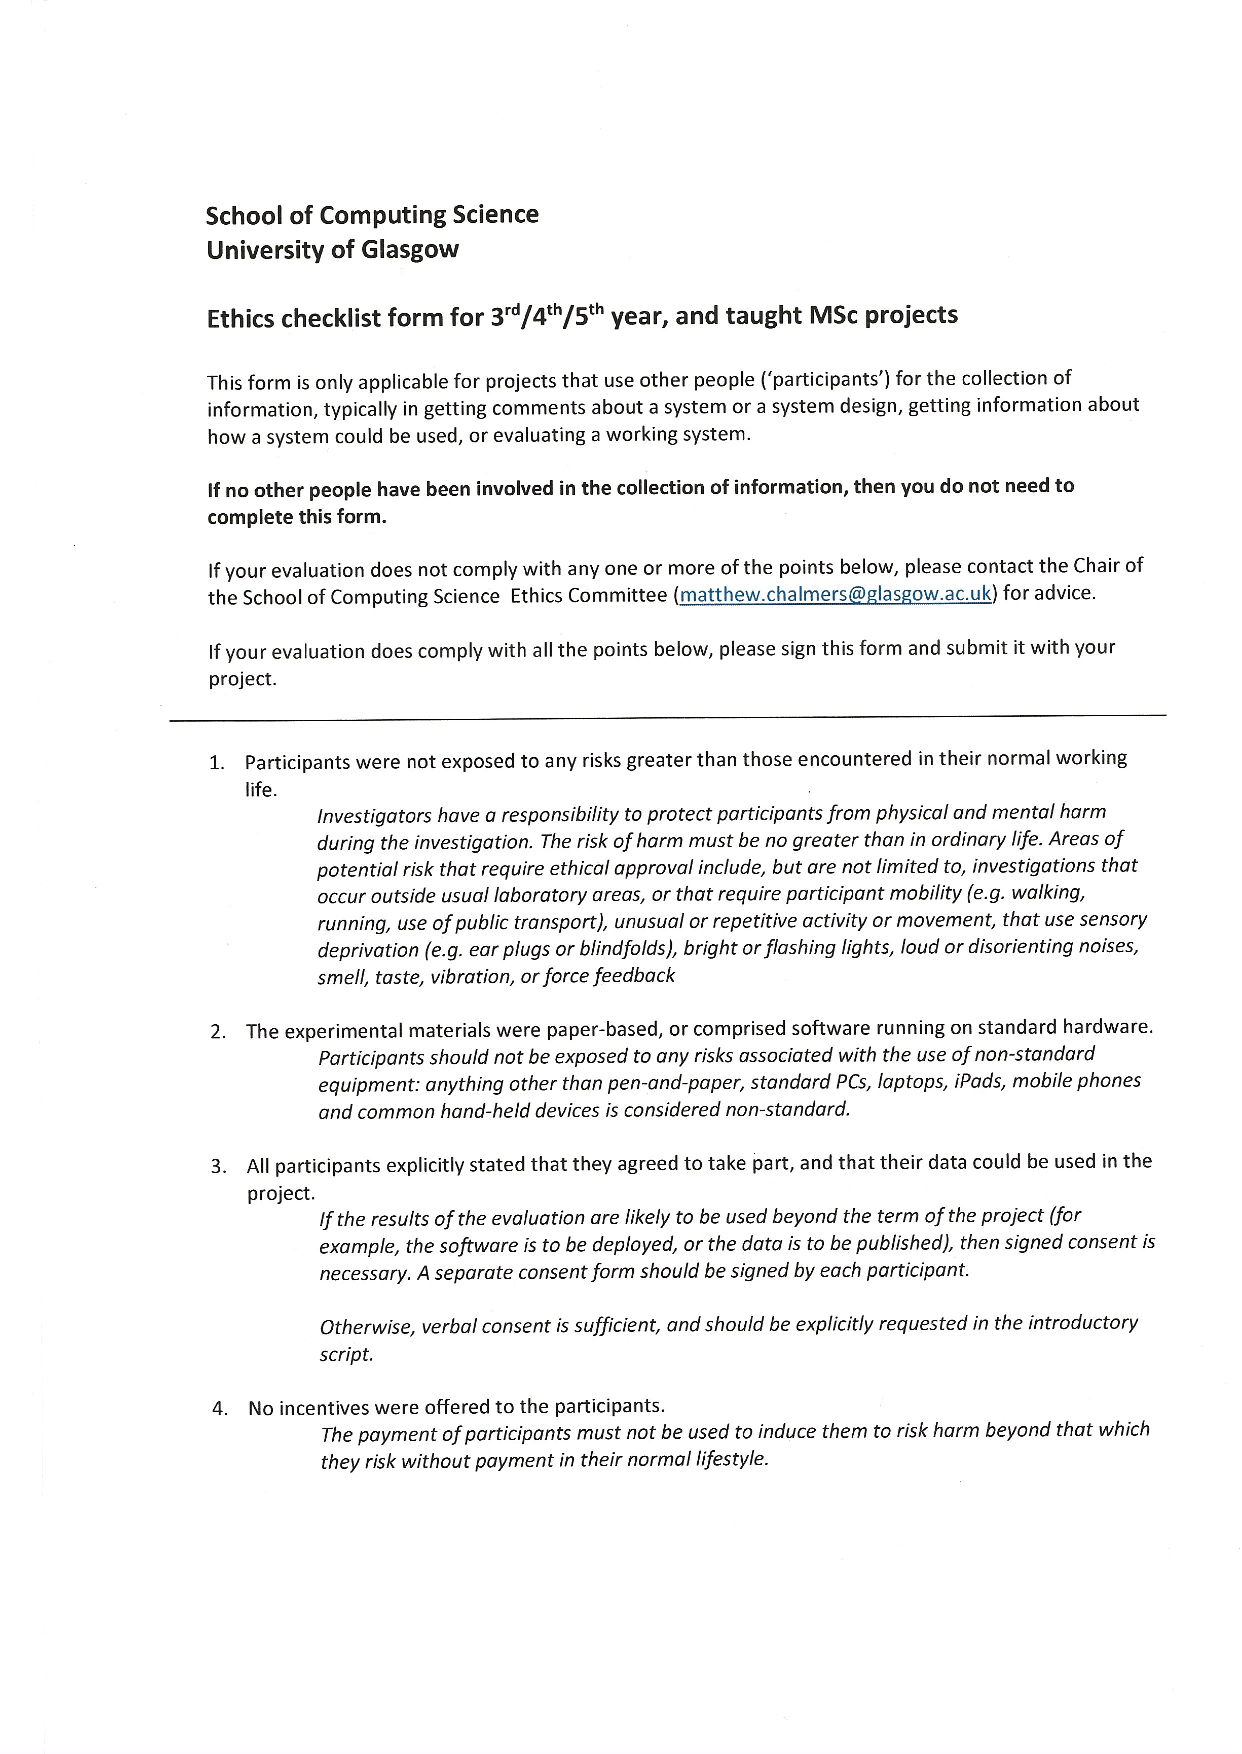
\includepdf[pages=-]{checklist.pdf}
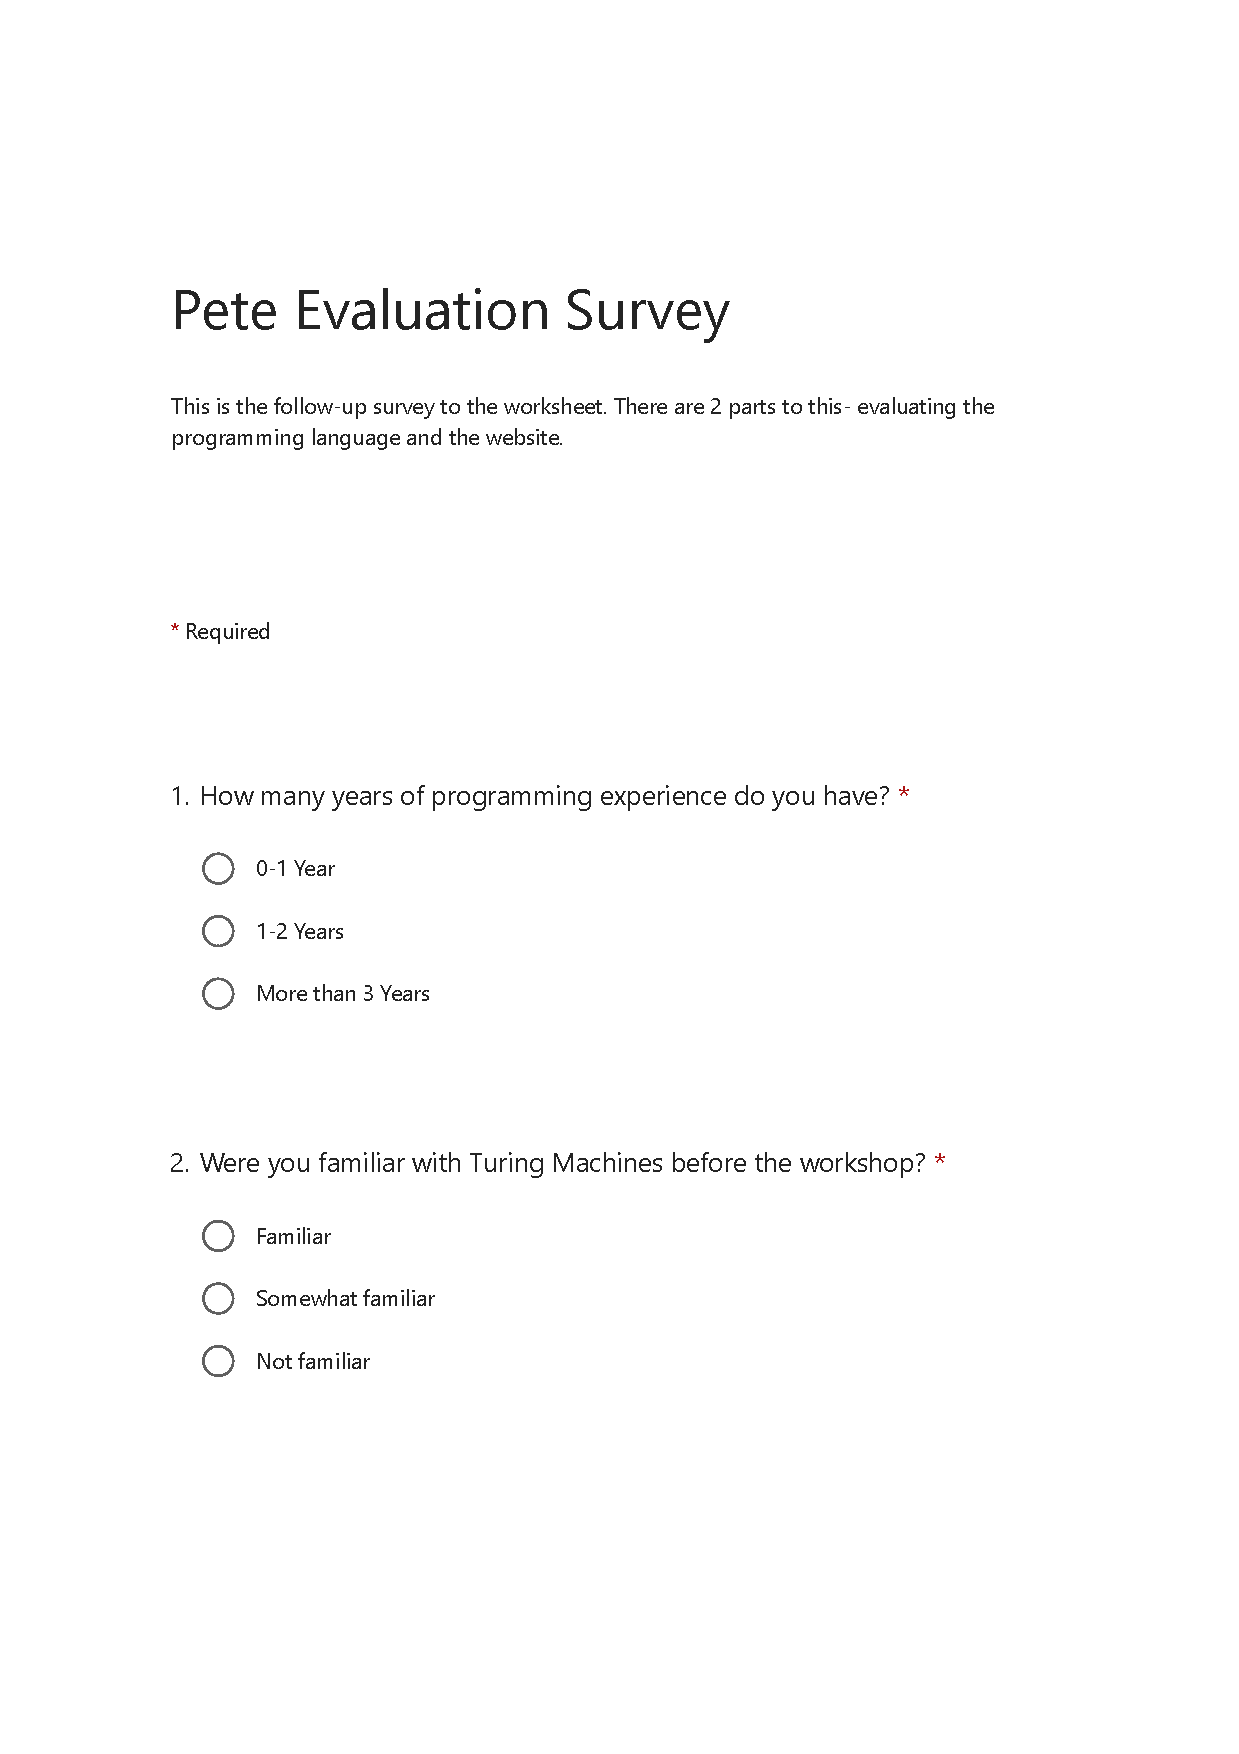
\includepdf[pages=-]{survey.pdf}

\end{appendices}